\section{Solar and Lunar Initiation}

\begin{quotex}
Christian initiation is the conscious experience of the heart of the world and the solar nature of man.
\flright{\textsc{Valentin Tomberg}}

If Hermetism has provided a safeguard for nearly twenty centuries, it must be said that circumstances have now changed. At the current point in history, as at the time of the Coming of Christ, the veil has been partially raised. Therefore, for those who want to advance beyond book knowledge, which never goes beyond the domain of information; for those who intensely seek the true sense of life, who want to understand the significance of the mission of the Christian in the New Era, the possibility will exist of initiation into this divine Wisdom, mysterious and hidden.  
\flright{\textsc{Boris Mouravieff}, \textit{Gnosis I}}

Classic initiation formula: \emph{try to grasp that which, once learned, you will know all}.
\flright{\textsc{Boris Mouravieff}, \emph{Gnosis II}}
\end{quotex}

\begin{wrapfigure}{rt}{.3\textwidth}
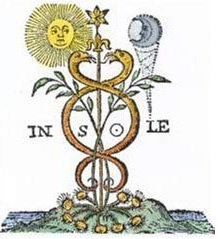
\includegraphics[width=.25\textwidth]{MarriageOfSunAndMoon.jpg}
\end{wrapfigure}

In his Meditation on the Lovers, Tomberg describes the experience of Initiation. Along the way, he teaches us how to understand symbolic texts. Commenting on the story of creation in Genesis, he points out that the true of that story lies not in its allegedly historical details --- viz., the Garden, Tree, Serpent, etc. --- but in our inner experience. By penetrating into the depths of the soul, one can recover a sense of the Primordial state and how it was lost. To make clear, this is not the same as some pseudo-intellectual description of symbols, but rather of conscious efforts to recreate that story in consciousness.

This, he says is knowledge of the ``beginning'', \emph{initium}, which knowledge is called initiation. As Mouravieff also points out, initiation now takes place on a spiritual plane, not on the material. Tomberg concurs, when he writes, ``God-man is the Initiator and there is no other.''

This descent into the depths of the human being is called Hermetic Initiation by Tomberg. Its method is enstasy, which is the aim of the jnani in the Vedantic systems. Following this path, the Initiate descends into the depths of his soul, until he awakens to the primordial layer of his soul as the ``image and likeness of God''. This is the alchemical creation of the true I or Will, the experience of the Microcosm.

The second type of initiation involves ecstasy, or the going outside oneself, leaving the Self behind to be absorbed in God or Heaven. This is what is commonly known as mystical experience. The Initiate reaches the beginning in terms of the Macrocosm. There is no need to discuss this at this point, since the literature is so vast.

However, it is the first type of initiation that is less known or even rejected when it is made known. However, in our time, when man has no experience of the Macrocosm nor even understands who he is, it is the necessary path. In the past, the development of the Self has been referred to as the Left Hand Path, in contrast to those paths that seek to annihilate the Self. Mouravieff goes so far as to point out the dangers of seeking ecstasy for its own sake. He points out that this often involves the use of drugs, or entheogens. Quite clearly, if the aim is consciousness of the Self and development of the Will, any drug induced stupor leads in the totally opposite direction.

For Mouravieff, then, the path of the Initiate in the Era of the Holy Spirit is the development of the I. Nevertheless, this does not preclude the experience of the Macrocosm as found in his elaborate cosmology, but rather that it must be done so consciously.

Tomberg insists the Christian esotericism unites the two paths. So, like the left hand paths, he proclaims the knowledge of the Self. Yet unlike those unbalanced deviations that see no more than material reality, Tomberg makes clear that the true Initiate must also be initiated in the right hand path. Table \ref{tab:SolarLunarInitiation} summarizes Tomberg's description of the two methods.

{\small
\begin{longtable}{p{.4\textwidth}p{.4\textwidth}}
\caption{Solar and Lunar Initiation}
\label{tab:SolarLunarInitiation}\\

\toprule
\textbf{Solar Initiation} & \textbf{Lunar Initiation} \\
\midrule
\endfirsthead

\toprule
\textbf{Solar Initiation} & \textbf{Lunar Initiation} \\
\midrule
\endhead

\midrule
\multicolumn{2}{r}{\textit{Continued on next page}}\\
\midrule
\endfoot

\bottomrule
\endlastfoot

Right Hand Path & Left Hand Path \\
Disciples of day & Disciples of night \\
Hermetic initiation & Pythagorean initiation \\
Conscious experience of the Initial microcosmic state & Conscious experience of the initial macrocosmic state \\
Conscious descent into the depth of the human being & Conscious ascent into the Empyrean \\
Enstasy & Ecstasy \\
Experience at the depths at the foundation within oneself & Rapture, or going out of oneself \\
One becomes more and more profound until one awakens within oneself to the primordial layer (the image and likeness of God) & The macrocosmic layers (spheres or heavens or Empyrean) reveal themselves to consciousness \\
The sense of spiritual touch & The sense of spiritual hearing \\
Like a chemical experiment undergone on the psychic and spiritual plane (alchemical and substantial) & Musical (music of the spheres) \& mathematical \\
Beginning is the microcosmic layer of Eden & Beginning is the macrocosmic sphere of Heaven \\
Sacred Heart (the intellectual center of man) & Cosmic Word (the Logos) \\

\end{longtable}
}

\textit{Originally published on 21 January 2012 on Medtarot.}


\flrightit{Posted on 2023-03-13 by Cologero}

\begin{center}* * *\end{center}

\begin{footnotesize}
\begin{sffamily}
\texttt{Kaukomieli on 2023-03-19 at 05:52 said:}

Hands that unite in prayer are the most intimate and clear expression of why the paths of the two hands should be united. Freedom and Love.

\end{sffamily}
\end{footnotesize}

